\documentclass{beamer}
\usepackage[autokw=all]{svn-multi}
\setbeamertemplate{navigation symbols}{}
%\usetheme{Goettingen}
\usetheme{Malmoe}
\usefonttheme{default}
%\setbeamersize{text margin left=5pt,text margin right=5pt}

\usepackage{hyperref}
\usepackage{subfigure}
\usepackage{amsmath}
\usepackage{amssymb}
\usepackage{multimedia}
\usepackage{shadow}
%\usepackage{movie15}

\usepackage{tcolorbox}

% Create a ``Wider'' command to reduce margins.  Put
% ``\Wider{\lipsum[2]}'' in a frame...
\newcommand\Wider[2][3em]{%
\makebox[\linewidth][c]{%
  \begin{minipage}{\dimexpr\textwidth+#1\relax}
  \raggedright#2
  \end{minipage}%
  }%
}


%\usepackage[english]{babel}
%\usepackage{pgf,pgfarrows,pgfnodes,pgfautomata,pgfheaps}
% \usepackage[latin1]{inputenc}

\usepackage{graphicx}
\defbeamertemplate*{footline}{default theme}
{
  \leavevmode%
  \hbox{%
  \begin{beamercolorbox}[wd=.5\paperwidth,ht=2.25ex,dp=1ex,center]{author in head/foot}%
    %\usebeamerfont{author in head/foot}\insertshortauthor~~(\insertshortinstitute)
    \usebeamerfont{author in head/foot}\insertshortauthor
  \end{beamercolorbox}%
  \begin{beamercolorbox}[wd=.4\paperwidth,ht=2.25ex,dp=1ex,center]{title in head/foot}%
    \usebeamerfont{title in head/foot}\insertshorttitle
  \end{beamercolorbox}%
  \begin{beamercolorbox}[wd=.1\paperwidth,ht=2.25ex,dp=1ex,right]{date in head/foot}%
%    \usebeamerfont{page number}\insertframenumber{} / \inserttotalframenumber\hspace*{2ex} 
    \usebeamerfont{page number}\insertpagenumber{} / \insertpresentationendpage{} \hspace*{2ex} 
  \end{beamercolorbox}}%
  \vskip0pt%
}

\title[$\alpha$go]{$\alpha$go}

\author{Ben Pearre}
%\institute[]{
%  Computer Science\\
%  University of Colorado at Boulder, USA}
\date{\today}
%\date{\today}

\begin{document}

\begin{frame}
  \titlepage
\end{frame}

\begin{frame}
  \frametitle{Outline}
  \tableofcontents
\end{frame}


%\begin{frame}
%  \outline
%\end{frame}


\section{Go}

\subsection{Rules}

\begin{frame}
  \frametitle{The Rules}
  \href{http://playgo.to/index-e.html}{\beamergotobutton{The Way To Go}}
\end{frame}

\subsection{How big is it?}

\begin{frame}
  \frametitle{How to win a game}
  \begin{itemize}
  \item Take best move on both sides until someone wins
  \item How many games?
    \begin{description}
    \item[Branching factor:] At each position, $n$ possible moves
    \item[Length:] game lasts $m$ moves
    \end{description}
    $n^m$ possible games
  \end{itemize}
\end{frame}


\begin{frame}
  \frametitle{Size of games}
  \begin{tabular}{l|ccc}
    Game & Branching factor & Length & $\log_{10}\mbox{\# Games}$\\ \hline
    Tic-Tac-Toe & 4 & 9 & 5 \\
    Connect Four & 4 & 36 & 21 \\
    Checkers ($8\times 8$) & 2.8 & 70 & 31 \\
    Chess & 35 & 70 & 108 \\
    Backgammon & 250 & 55 & 132 \\
    Carcassonne & 55 & 71 & 195 \\
    Go & 250 & 150 & 360
  \end{tabular}
\end{frame}


\section{Game theory}

\subsection{Minimax search}

\begin{frame}
  \frametitle{Reducing the computational complexity}
  \begin{description}
  \item[Branching factor]:\hfill
    \begin{itemize}
    \item Pruning (e.g. $\alpha$-$\beta$)
    \item Monte Carlo tree search
    \end{itemize}
  \item[Length:]\hfill
    \begin{itemize}
    \item Estimate the value of non-terminal states
    \end{itemize}
  \end{description}
  How to approximate these things?
\end{frame}


\begin{frame}
  \frametitle{Static Evaluation}
  \begin{description}
  \item[Checkers:]\hfill
    \begin{itemize}
    \item Material
    \item Position of non-kings
    \end{itemize}
  \item[Chess:]\hfill
    \begin{itemize}
    \item Control centre of board
    \item Material
    \end{itemize}
  \item[Go:]\hfill
    \begin{itemize}
    \item ``Strength'' / ``Influence''
      \begin{itemize}
      \item Um\dots
      \end{itemize}
    \end{itemize}
  \end{description}
\end{frame}

\begin{frame}
  \frametitle{Move selection}
  Only examine promising moves.
  \begin{tcolorbox}
    In the beginner's mind there are many possibilities. In the expert's mind there are few.
  \end{tcolorbox}
  How to build an expert?
\end{frame}



\subsection{Convolutional neural networks}

\begin{frame}
  \frametitle{Neural Networks}
  \begin{columns}
    \begin{column}{0.5\textwidth}
      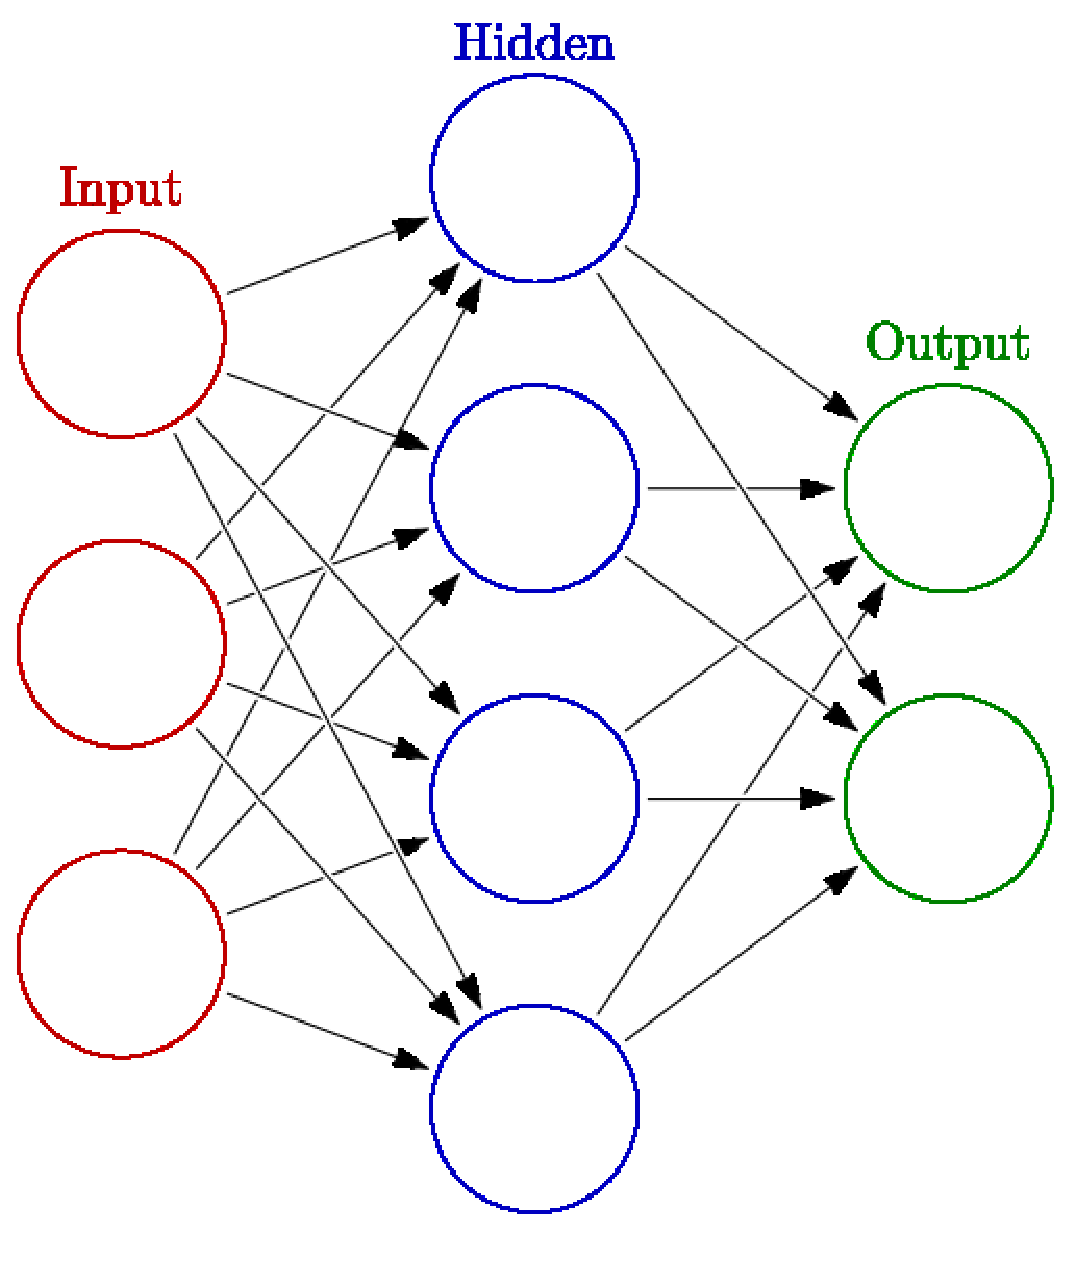
\includegraphics[width=0.8\textwidth]{neural_network}
    \end{column}
    \begin{column}{0.5\textwidth}
      \begin{itemize}
      \item Input pattern $\xi$
      \item Weights $W$
      \item $y = W_1 \tanh (W_0 \xi) $
      \item $W_i$ are trained with backpropagation of errors
      \end{itemize}
    \end{column}
  \end{columns}
\end{frame}

\begin{frame}
  \frametitle{Convolutional Neural Networks}
  \vskip 1 cm
  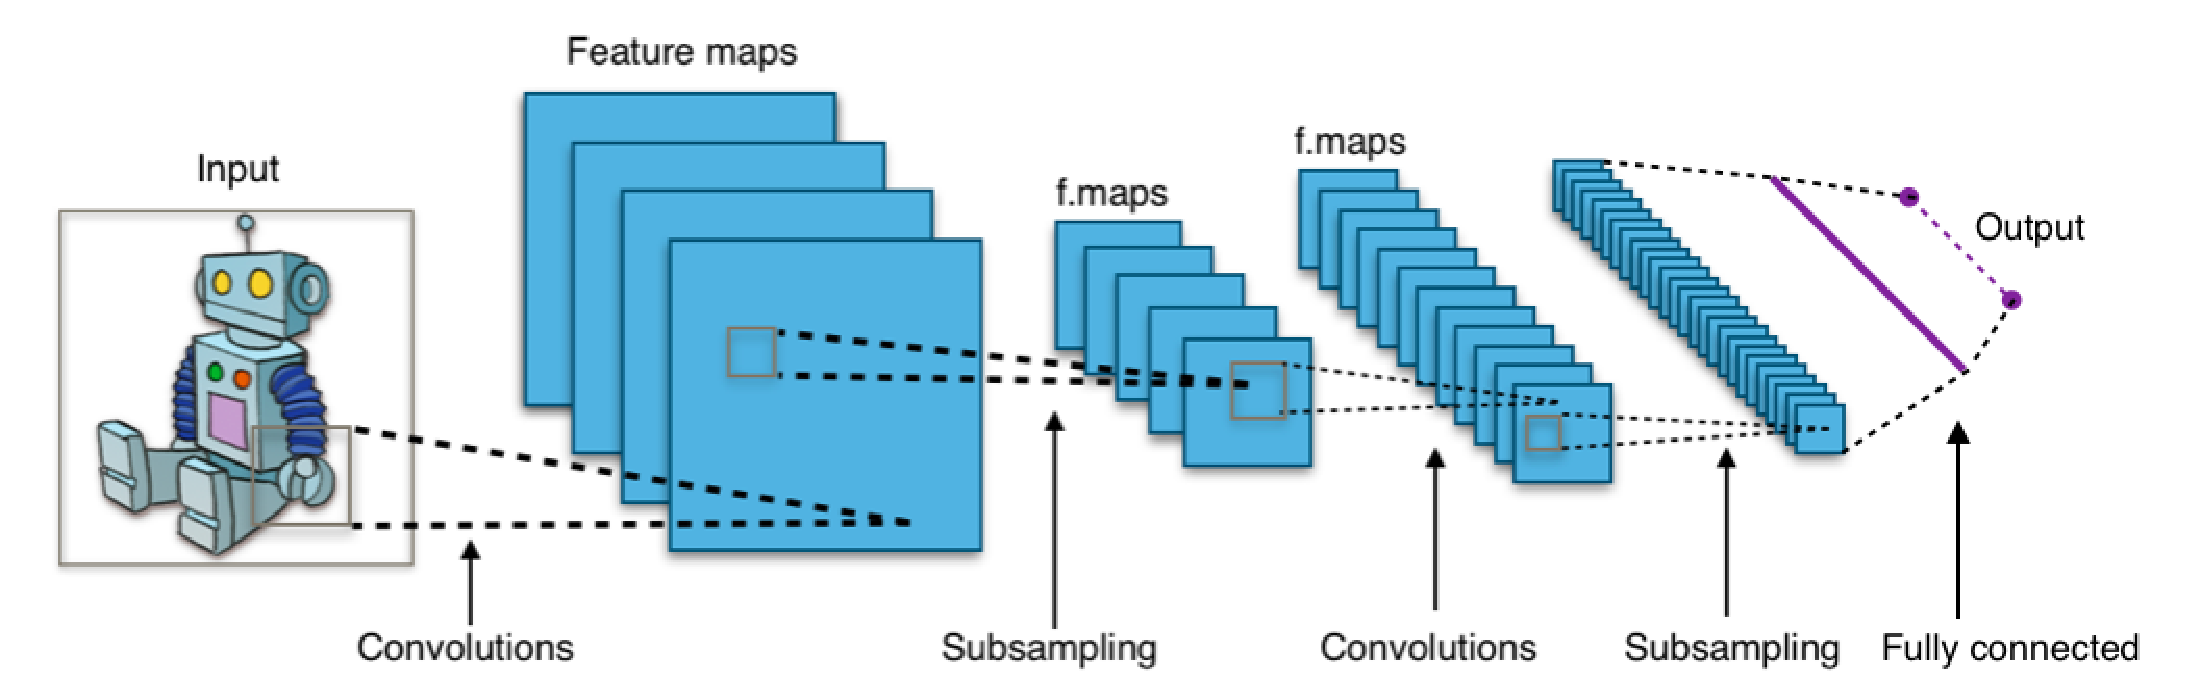
\includegraphics[width=\textwidth]{ConvolutionalNet}

  \vskip 1 cm
  \begin{center}
    \href{http://yann.lecun.com/exdb/lenet/}{\beamergotobutton{LeNet}}
  \end{center}
\end{frame}

\begin{frame}
  \frametitle{Supervised learning of policy networks: $p_\sigma(a|s)$}
  Predict the expert's move:
  \begin{itemize}
  \item Given board state $s$, predict probability of move $a$
  \item 13 convolutional layers
    \begin{itemize}
    \item Input: 48 feature planes
    \item Layer 1: 192 of $5\times 5$
    \item Layers 2--12: 192 of $3\times 3$
    \item Rectifier nonlinearities
    \end{itemize}
  \item Training: 30 million positions from KGS
  \item 57\% accurate
  \item Evaluation time: 3 ms
  \end{itemize}
  \begin{tcolorbox}
    \begin{center}
      $\Delta \sigma \propto \frac{\partial \log p_\sigma(a_t|s_t)}{\partial \sigma}$
    \end{center}
  \end{tcolorbox}
\end{frame}

\begin{frame}
  \frametitle{Supervised learning of policy networks II: $p_\pi(a|s)$}
  Predict the expert's move:
  \begin{itemize}
  \item Given board state $s$, predict probability of move $a$
  \item Small pattern features
  \item Training: 8 million positions from Tygem (?)
  \item 24\% accurate
  \item Evaluation time: 2 $\mu$s
  \end{itemize}
  Why? To be continued\dots
\end{frame}

\begin{frame}
  \frametitle{Reinforcement learning of policy networks: $p_\rho(a|s)$}
  Don't predict expert moves: Win!
  \begin{itemize}
  \item Start with the supervised move predictor: $\rho \leftarrow \sigma$
  \item Training: self-play vs. a previous iteration of $\rho$
  \item Result of game is $z$
  \end{itemize}
  \begin{tcolorbox}
    \begin{center}
      $\Delta \rho \propto \frac{\partial \log p_\rho(a_t|s_t)}{\partial \rho}z$
    \end{center}
  \end{tcolorbox}
  $p_\rho$ won 80\% of its games vs. $p_\sigma$
\end{frame}


\begin{frame}
  \frametitle{Reinforcement learning of value networks: $v^p(s)$}
  Predict the likelihood of winning from any board position
  \begin{itemize}
  \item $v^p(s) = \mathbb{E}\left[ z | s = s_t, a_{t\ldots T} \sim p\right]$
  \item Similar architecture to $p_\rho$, but outputs scalar $v$
  \item Trained from 30 million samples from self-play by $p_\rho(s,a)$
    \begin{itemize}
    \item Decorrelate sequences of moves
    \end{itemize}
  \end{itemize}
  \begin{tcolorbox}
    \begin{equation*}
      \Delta \theta \propto \frac{\partial v_\theta(s)}{\partial \theta}(z-v_\theta(s))
    \end{equation*}
  \end{tcolorbox}
\end{frame}




\section{Move selection}


\begin{frame}
  \frametitle{Evaluating a potential move}
  \begin{itemize}
  \item Choose action $a$ from $p_\sigma$ + exploration term
  \item Evaluate new position 2 ways:
    \begin{itemize}
    \item $v_\theta(s)$
    \item Monte Carlo rollout using the fast policy $p_\pi$
    \end{itemize}
    \item Combine the evaluations
  \end{itemize}
  \vskip 1 cm
  \begin{tcolorbox}
    \begin{center}
      Choose the most visited move!
    \end{center}
  \end{tcolorbox}
\end{frame}


\begin{frame}
  \frametitle{Monte Carlo Tree Search}
  New node: get priors from $p_\sigma(s,a)$ + exploration term
  \vskip 5 mm
  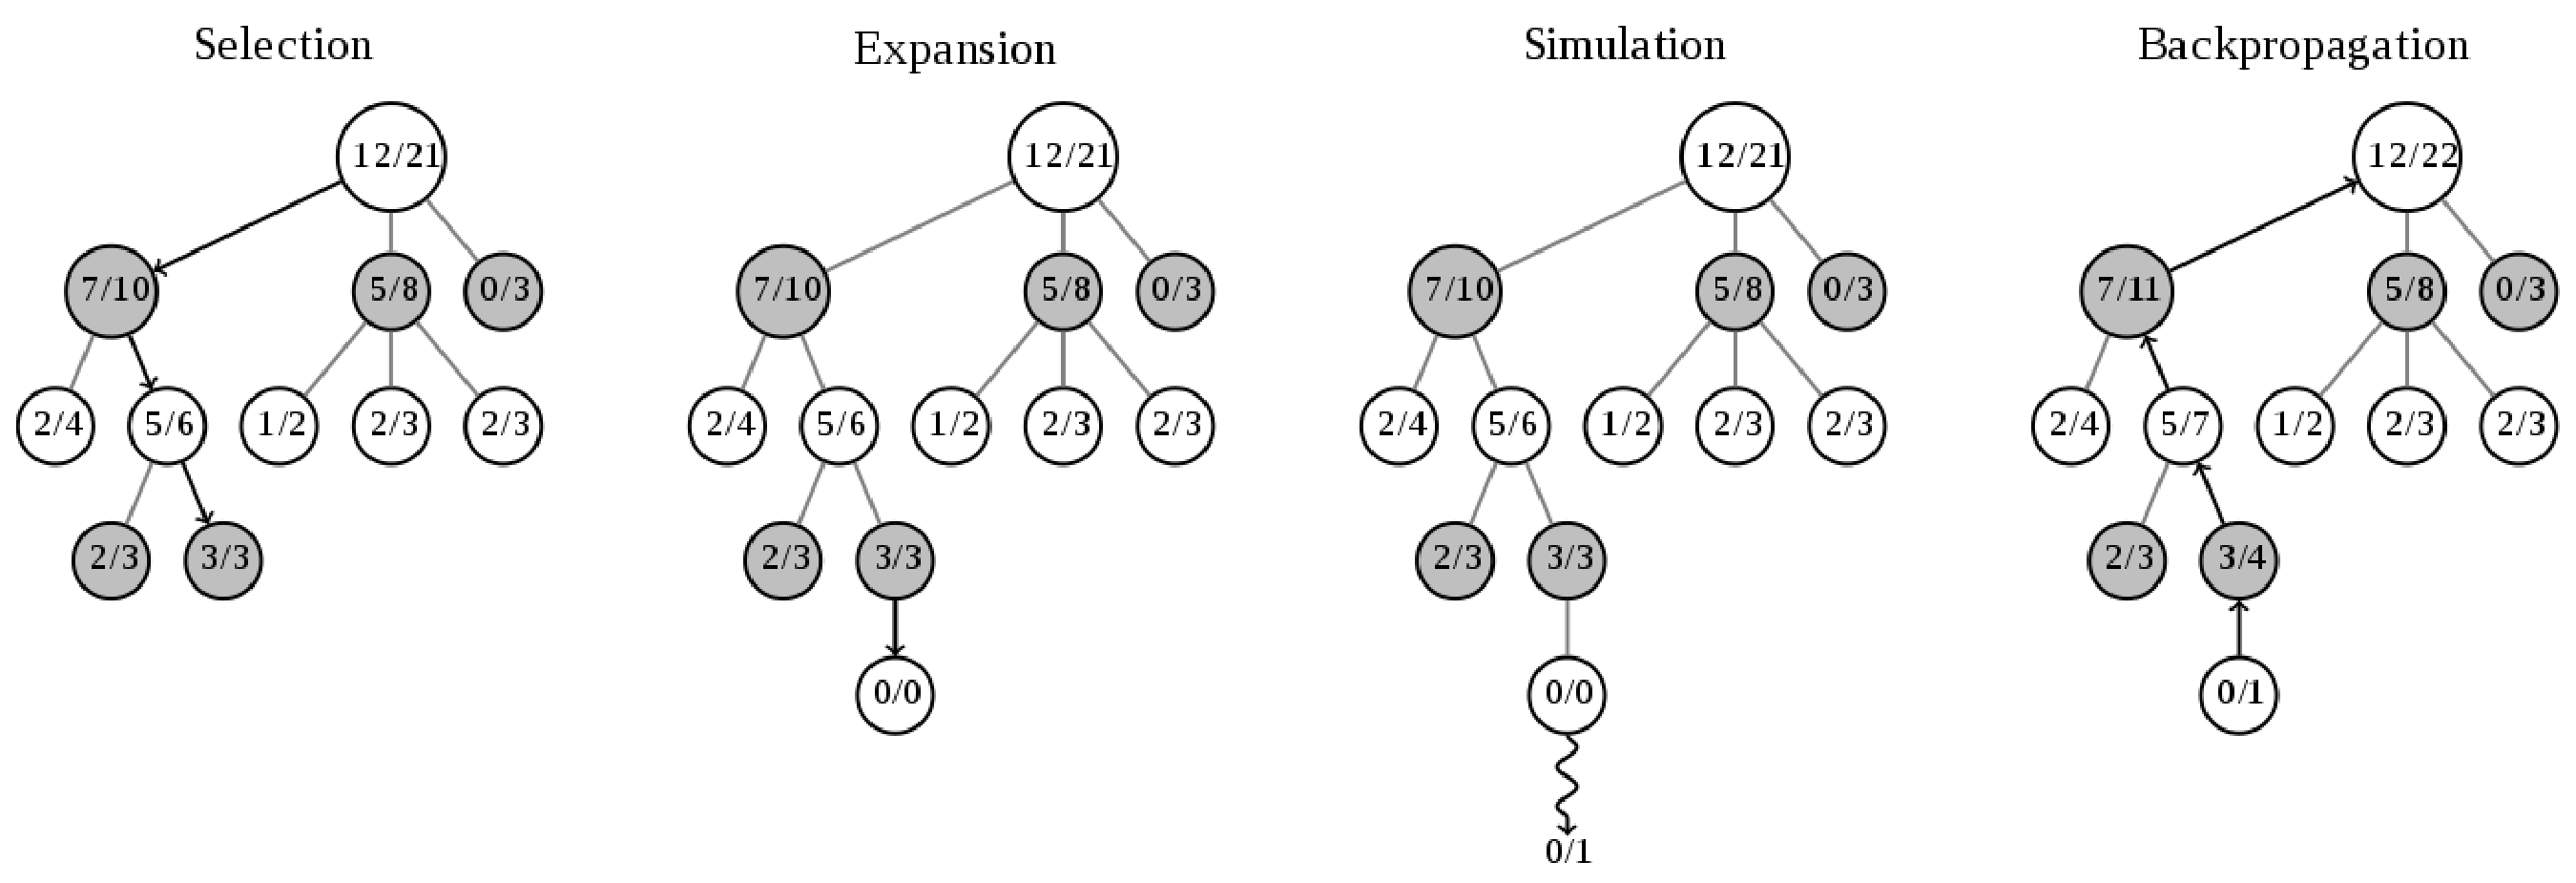
\includegraphics[width=\textwidth]{MCTS}
  \begin{columns}
    \column{0.5\textwidth}
    Early:
    \begin{itemize}
    \item High prior probability
    \item Low visit count
    \end{itemize}
    \column{0.5\textwidth}
    Later:
    \begin{itemize}
    \item High action value
    \end{itemize}
  \end{columns}
\end{frame}

\section{Results}

\begin{frame}
  \frametitle{Results}
  \begin{itemize}
  \item Beat Lee Sedol 9p 4-1
  \item $10^3$ times fewer position evaluations than Deep Blue!
    \begin{itemize}
    \item Learns to aggressively examine only a few promising moves
    \item Learns intuition for values of intermediate positions
    \item Plays like a human?
    \end{itemize}
  \end{itemize}
\end{frame}


\end{document}
